\subsection{Anwendungen}
\subsubsection{Elektrotechnik}
Was braucht man:

\begin{minipage}[T]{0.49\textwidth}
    \begin{circuitikz}
        \draw (0,5) to [R, l_=$R$] +(4.5,0);
        \draw (0,2.5) to [C, l_=$C$] +(4.5,0);
        \draw (0,0) to [L, l=$L$] +(4.5,0);
    \end{circuitikz}
\end{minipage}
\begin{minipage}{0.49\textwidth}
    \begin{equation*}
        U_R =R\cdot i=R\cdot\dot{q}
    \end{equation*}
    
    \vspace{1em}
    \begin{equation*}
        U_C = \frac{1}{C}\int i dt = \frac{1}{C}q
    \end{equation*}
    oder
    \begin{equation*}
        \dot{U_C}=\frac{1}{C}i
    \end{equation*}

    \vspace{2em}
    \begin{equation*}
        U_L = L\cdot \frac{di}{dt}=L\ddot{q}
    \end{equation*}

\end{minipage}

\definition{Knotenregel}{In einem Knotenpunkt ist die Summe der zu- und \\abflies\-senden Ströme gleich null}

\begin{center}\begin{tikzpicture}
    \draw (0,0) -- (1,0) node[midway,below] {$\rightarrow I_1$} -- ++(0,1) -- ++(2,0) node[midway,below] {$\rightarrow I_2$} ;
    \draw (1,0) -- ++(0,-1) -- ++(2,0) node[midway,above] {$\rightarrow I_3$}; 
    \fill (1,0) circle[radius=0.1];
    \node at (6,0) {$I_1 + I_2 + I_3 =0 $};
\end{tikzpicture}\end{center}

\definition{Maschenregel}{In jeder Masche ist die Summe der Spannungen gleich 0}

%\begin{center}\begin{circuitikz}
%\draw (0,0) to (0,1) to [R,l=$R$] (3,1) to (3,0) to [L,l=$L$] (0,0);
%\node at (6,0.5) {$U_R+U_L=0$};
%\end{circuitikz}\end{center}

\bsp{Beispiel: Kondensator-Entladung}
\begin{center}\begin{circuitikz}
    \draw   (0,0) to [R, l_=$R$] ++(5,0) 
            -- ++(0,2)
            to [C, l=$C$] ++(-5,0)
            -- (0,0);
\end{circuitikz}\end{center}
Kondensator anfänglich geladen auf $Q_0$\\
$Q=C\cdot U \rightarrow U_0 = \frac{Q_0}{C}$

Maschenregel:
\begin{equation*}
    U_R+U_C=0
\end{equation*}

Es gibt 3 Möglichkeiten, die DGL aufzustellen:

\begin{outline}
    \1[a)] Strom
    \begin{eqnarr}
        U_R + U_C &=& 0 \\
        &\Rightarrow&\\ 
        R\cdot i + \frac{1}{C}\int i dt &=& 0\hspace{2em}\left|\frac{d}{dt}\right.\\
        R\frac{\partial i}{\partial t} + \frac{1}{C} i &=& 0,\hspace{2em} i\left( 0 \right) = \frac{1}{R}U_0
    \end{eqnarr}

    \1[b)] Ladung
    \begin{eqnarr}
        U_R + U_C &=& 0 \\
        &\Rightarrow&\\ 
        R\cdot \dot{q} + \frac{1}{C}q &=& 0,\hspace{2em} q\left( 0 \right) = C\cdot U_0
    \end{eqnarr}

    \1[c)] Spannung (am Kondensator)
    \begin{equation*}
        U_R + U_C = 0
    \end{equation*}
    Ausnützen dass der Strom im Kondensator und im Widerstand gleich sind: $i_R=i_C$:
    \begin{eqnarr}
        U_R &=& R\cdot i\\
        &=& R\cdot \left( C\cdot \dot{U}_C \right) \\
        &\Rightarrow&\\
        R\cdot C\cdot \dot{U}_C + U_C &=& 0,\hspace{2em} U_C\left( 0 \right) = U_0
    \end{eqnarr}
        
\end{outline}

\subsubsection{Mechanik}
a) ohne Schwingungen

Bewegungsgleichungen
\begin{center}\begin{tabular}{lcc}
\toprule
&Lineare Bewegung&Drehbewegung \\
\midrule
Ort & $s(t)$& $\varphi (t)$ \\
Geschw. &$v(t)=\dot{s}$& $\omega(t) = \dot{\varphi} $\\
Beschl. &$a(t)=\dot{v}=\ddot{s}$&$\alpha(t) = \dot{\omega}=\ddot{\varphi}$ \\
\bottomrule
\end{tabular}\end{center}

\definition{Bewegungsgesetz von Newton}{Beschleunigung  = Summe aller \\angreifenden Kräfte geteilt durch Masse}
\begin{eqnarr}
    m\a &=&  m \ddot{\vec{s}} = \sum \vec{F}_i \\
    J\vec{\alpha} &=&  m \ddot{\vec{\varphi}} = \sum \vec{M}_i \\
\end{eqnarr}

\definition{Kräftezerlegung}
{Das Bewegungsgesetz von Newton gilt in einem \\senkrechten Koordinatensystem für alle Komponenten einzeln.}
\begin{center}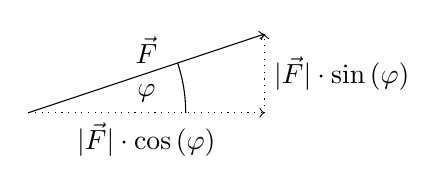
\begin{tikzpicture}
    \draw[->] (0,0) -- (3,1) node[midway,above] {$\vec{F}$};
    \draw[->,dotted] (0,0) -- (3,0) node[midway,below] {$|\vec{F}|\cdot \cos \left( \varphi \right)$};
    \draw[->,dotted] (3,0) -- (3,1) node[midway,right] {$|\vec{F}|\cdot \sin \left( \varphi \right)$};
    \draw (2,0) arc (0:18.43:2);
    \node at(1.5,0.25) {$\varphi$};
\end{tikzpicture}\end{center}

\bsp{Beispiel}
Freier Fall ohne Reibung
\begin{eqnarr}
        m\cdot a&=& -g \cdot m\\
        \ddot{y} &=& -g\\
        \dot{y} &=& -g\cdot t + v_0\\
        y &=& -\frac{1}{2}\cdot g\cdot t^{2} + v_0 \cdot t+y_0
\end{eqnarr}

\subsubsection*{Kräfte}
\definition{Schwerkraft}{$F_G=g\cdot m$}
\definition{Coulombsche Reibung}{Trockene Reibung: $F_R=-\mu \cdot F_N$}
\definition{Stokes Reibung}{In Flüssigkeiten (Re klein) $F_R=-\mu \cdot v$}
\definition{Newton Reibung}{In Luft (Re gross) $F_R=-\mu\cdot\mbox{sign} \left( v \right)\cdot v^{2}$}

Wichtig: Reibkraft immer der Geschwindigkeit entgegengerichtet.

\bsp{Beispiel Schiefe Ebene:}
\begin{center}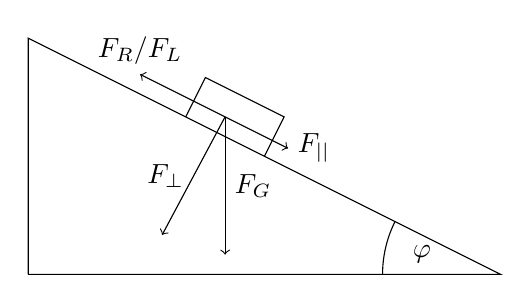
\begin{tikzpicture}
    \draw (0,0) -- (6,0) -- (0,3) -- (0,0);
    \draw (3,1.5) -- ++(0.25,0.5) -- ++(-1,0.5) -- ++(-0.25,-0.5);
    \draw[->] (2.5,2) -- ++(0,-1.75) node[midway,right] {$F_G$};
    \draw[->] (2.5,2) -- ++(-0.8,-1.5) node[midway,left] {$F_\bot$};
    \draw[->] (2.5,2) -- ++(0.8,-0.4) node[right] {$F_{||}$};
    \draw[->] (2.5,2) -- ++(-1.08,0.54) node[above] {$F_{R}/F_L$};
    \draw (4.5,0) arc (180:180-26.6:1.5);
    \node at (5,0.25) {$\varphi$};
\end{tikzpicture}\end{center}
\begin{IEEEeqnarray*}{lrCl}
    \mbox{Schwerkraft:}\hspace{2em} & F_G &=& m\cdot g\\
    & F_{||} &=& m\cdot g \cdot \sin\left( \varphi \right)\\
    & F_{\bot} &=& m\cdot g \cdot \cos\left( \varphi \right) \\
    \mbox{Luftreibung:}\hspace{2em} & F_L &=& -k\cdot v^{2}\\
    \mbox{Haftreibung:}\hspace{2em} & F_R &=& -\mu\cdot F_\bot\\
    & &=& -\mu\cdot m\cdot g\cdot\cos\left( \varphi \right)
\end{IEEEeqnarray*}
In die Bewegungsgleichung einsetzen
\begin{eqnarr}
    m\cdot a &=& \sum F \\
    m \cdot a &=& F_{||} + F_L + F_R\\
    &=&  m\cdot g \cdot \sin\left( \varphi \right) -k\cdot v^{2}
    -\mu\cdot m\cdot g\cdot\cos\left( \varphi \right)\\
    &=&  m\cdot g \cdot \left( \sin\left( \varphi \right) - 
         \mu\cdot\cos\left( \varphi\right)  \right)
         - k\cdot v^{2}\\
     &\Rightarrow& \\
     m\cdot\dot{v} + k\cdot v^{2} &=&  m\cdot g \cdot 
     \left( \sin\left( \varphi \right) - 
         \mu\cdot\cos\left( \varphi\right)  \right)
\end{eqnarr}
Nichtlineare, nicht Elementar lösbare, inhomogene (mit konstanten Koeffizienten) und gewöhnliche DGL 1. Ordnung.



b) mit Schwingungen

Eine Schwingung kommt dann zustande, wenn es eine vom Ort abhängige, rücktreibende Kraft gibt.\\
Zusätzliche Kräfte:
\definition{Federkraft}{
(Hooksches Gesetz)
\begin{equation*}
F = - k \cdot x
\end{equation*}}
\definition{Dämpfer}{
(Reibkraft in einer Schwingung)
\begin{equation*}
    F = - \gamma \cdot \dot{x}
\end{equation*}}


\bsp{Beispiel Physikalisches Pendel:}

\begin{minipage}{0.3\linewidth}
\begin{center}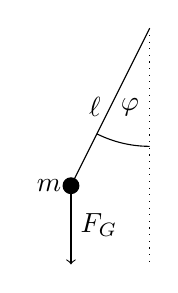
\begin{tikzpicture}
    \draw (0,0) -- (-1,-2) node[midway,left] {$\ell$} node[left] {$m$} [fill] circle[radius=0.1];
    \draw[->] (-1,-2) -- ++ (0,-1) node[midway,right] {$F_G$};
    \draw[dotted] (0,0) -- (0,-3);
    \draw (0,-1.5) arc (270:270-26.6:1.5);
    \node at (-0.25,-1) {$\varphi$};
\end{tikzpicture}\end{center}
\end{minipage}
\begin{minipage}{0.6\linewidth}
    \begin{IEEEeqnarray*}{lrCl}
        \mbox{Trägheitsmoment:}\hspace{1em} & J &=&  m\cdot \ell^{2} \\
        \mbox{Drehmoment:} & M &=& m\cdot g\cdot\sin\left(\varphi\right)\cdot\ell 
    \end{IEEEeqnarray*}
\end{minipage}

In die Bewegungsgleichung einsetzen
\begin{eqnarr}
    J\cdot \ddot{\varphi} &=& \sum M \\
    &\Rightarrow& \\
    m\cdot\ell^{2}\cdot\ddot{\varphi} &=&  m\cdot g\cdot\sin\left(\varphi\right)\cdot\ell \\
    &\Rightarrow& \\
    \ell\ddot{\varphi} - g\sin\left( \varphi \right) &=& 0\\
\end{eqnarr}
Für kleine $\varphi$ gilt $\sin\left( \varphi \right) \approx \varphi\Rightarrow$
\begin{equation*}
    \underbrace{\ell\ddot{\varphi} - g\varphi}_\text{Schwingungsgleichung}= 0
\end{equation*}

\subsubsection{Bilanzgleichungen}
(Kalkül mit Differentialen)
\begin{center}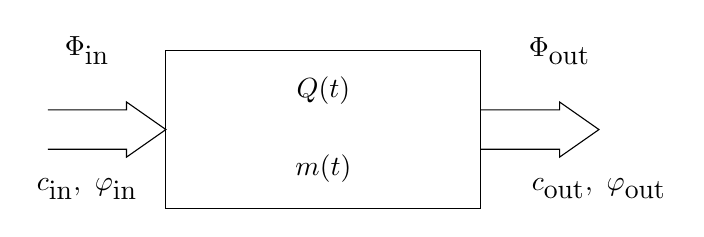
\begin{tikzpicture}[scale=1]
    \draw (0,0) rectangle (4,2);
    \draw (-1.5,0.75) --++ (1,0) --++ (0,-0.1) --++ (0.5,0.35)
          --++(-0.5,0.35)--++(0,-0.1)--++(-1,0);
    \draw (4,0.75) --++ (1,0) --++ (0,-0.1) --++ (0.5,0.35)
          --++(-0.5,0.35)--++(0,-0.1)--++(-1,0);
    \node at (-1,2) {$\Phi_{\mbox{in}}$};
    \node at (-1,0.25) {$c_{\mbox{in}},~\varphi_{\mbox{in}}$};
    \node at (5,2) {$\Phi_{\mbox{out}}$};
    \node at (5.5,0.25) {$c_{\mbox{out}},~\varphi_{\mbox{out}}$};
    \node at (2,1.5) {$Q(t)$};
    \node at (2,0.5) {$m(t)$};
\end{tikzpicture}\end{center}

\begin{IEEEeqnarray*}{rClCl}
    \Phi &:& \mbox{Fluss} &:& \left[ \frac{\mbox{Menge, Vol}}{\mbox{Zeit}}
    \right]\\
    \varphi &:& \mbox{Volumenfluss} & & \\
    c &:& \mbox{Konzentration} &:& \left[ \frac{\mbox{kg}}{\si{m^3}} \right]
\end{IEEEeqnarray*}

\bsp{Beispiel 1 Alkoholtank}

Ein \SI{1000}{l} Tank ist gefüllt mit mit 80\% Alkohol. Mit einer Füllrate
von \SI{10}{l/min} wird 60\% Alkohol nachgefüllt und gut gemischt. Die
gleiche Menge fliesst aus.

\begin{center}\begin{tikzpicture}[scale=2]
    \draw (0,0) -- ++(6,0);
    \draw (0,0.25) -- ++(2,0) -- ++(0,2) -- ++(2,0) -- ++(0,-2) --++(2,0);
    \node at (0.5,0.75) {$\Phi_{\mbox{in}}=\SI{10}{l/min}$};
    \node at (0.5,0.4) {$\dot{m}_{\mbox{in}}=c\cdot\Phi$};
    \node at (0.5, -0.25) {60\%};
    \node at (3, 1.5) {\SI{1000}{l}};
    \node at (3, 1) {$a(t)$: Alkoholmenge};
\end{tikzpicture}\end{center}


\begin{eqnarr}
    \Delta a &=& 10 \cdot 0.6 \Delta t - 10 \cdot \frac{a(t)}{1000}\Delta t \\    
    \Delta a &=& \left( 6-\frac{a(t)}{100} \right)\Delta t \\
    \frac{\Delta a}{\Delta t} &=&  6 - \frac{a(t)}{100} \\
    \Delta t \rightarrow 0 &\Rightarrow& \\
    \dot{a}(t) &=&  6 -\frac{a(t)}{100}
\end{eqnarr}

$\Rightarrow$ Die Alkoholmenge $a(t)$ wird durch die Differentialgleichung
$\dot{a}(t) =  6 -\frac{a(t)}{100}$ beschrieben. Zusammen mit der
Anfangsbedingung $a(0) = 800$ ergibt sich das entsprechende Anfangswertproblem.

\bsp{Beispiel 2 Bakterienkultur}

Eine Bakterienkultur enthält eine Menge $x(t)$ Bakterien. Sie wächst mit 
einer Geschwindigkeit proportional zu der Anzahl bereits vorhandenen Bakterien.

\begin{eqnarr}
    \Delta x &=&  \lambda x(t) \Delta t \\
    \frac{\Delta x}{\Delta t} &=&  \lambda x(t) \\
    \dot{x}(t) &=&  \lambda x(t)
\end{eqnarr}

Diese DGL hat die allgemeine Lösung $x(t) = Ce^{\lambda t}$
